\subsection{Summary and Recommendations}

Based on our comprehensive analysis of both KNN and SVM classifiers across the mushroom and hepatitis datasets, we can make several dataset-specific recommendations while considering the inherent tradeoffs between these algorithms.

\paragraph{Mushroom Dataset}
For the mushroom classification task, both KNN and SVM demonstrated strong performance, with SVM showing a slight edge in overall accuracy. The key findings include:

\begin{itemize}
    \item SVM achieved perfect classification accuracy (100\% F1 score) with polynomial and RBF kernels
    \item KNN performed well but required more careful tuning of the k parameter
    \item Both polynomial and RBF kernels in SVM proved highly effective
\end{itemize}

\textbf{Recommendation:} For the mushroom dataset, we recommend using SVM with either a polynomial kernel ($C=5$ or $C=50$) or RBF kernel ($C=50$) as the primary classifier.

\paragraph{Hepatitis Dataset}
The hepatitis classification task revealed different characteristics:

\begin{itemize}
    \item KNN showed more robust performance across different parameter configurations
    \item SVM required more careful kernel selection and parameter tuning
    \item The smaller dataset size made KNN's memory requirements less problematic
\end{itemize}

\textbf{Recommendation:} For the hepatitis dataset, we recommend KNN as the primary classifier, particularly with k values between 3 and 5. The decision is based on its robust performance and simpler implementation requirements.

\paragraph{Instance Reduction Considerations}
The application of instance reduction techniques, particularly GCNN, demonstrated significant benefits for computational efficiency:

\begin{itemize}
    \item For the mushroom dataset, GCNN achieved substantial reductions in testing time for KNN, with approximately 50\% faster predictions
    \item Storage requirements were notably decreased, especially beneficial for the larger mushroom dataset
    \item However, some reduction methods (particularly Drop3) showed slight decreases in classification performance
    \item The hepatitis dataset saw more modest improvements, likely due to its already small size, and reduction made performance worse
\end{itemize}

\textbf{Recommendation:} Consider applying GCNN reduction when working with larger datasets where prediction speed is crucial and minor accuracy trade-offs are acceptable. For smaller datasets like hepatitis, the benefits may not justify the potential accuracy loss.

\begin{figure}
    \centering
    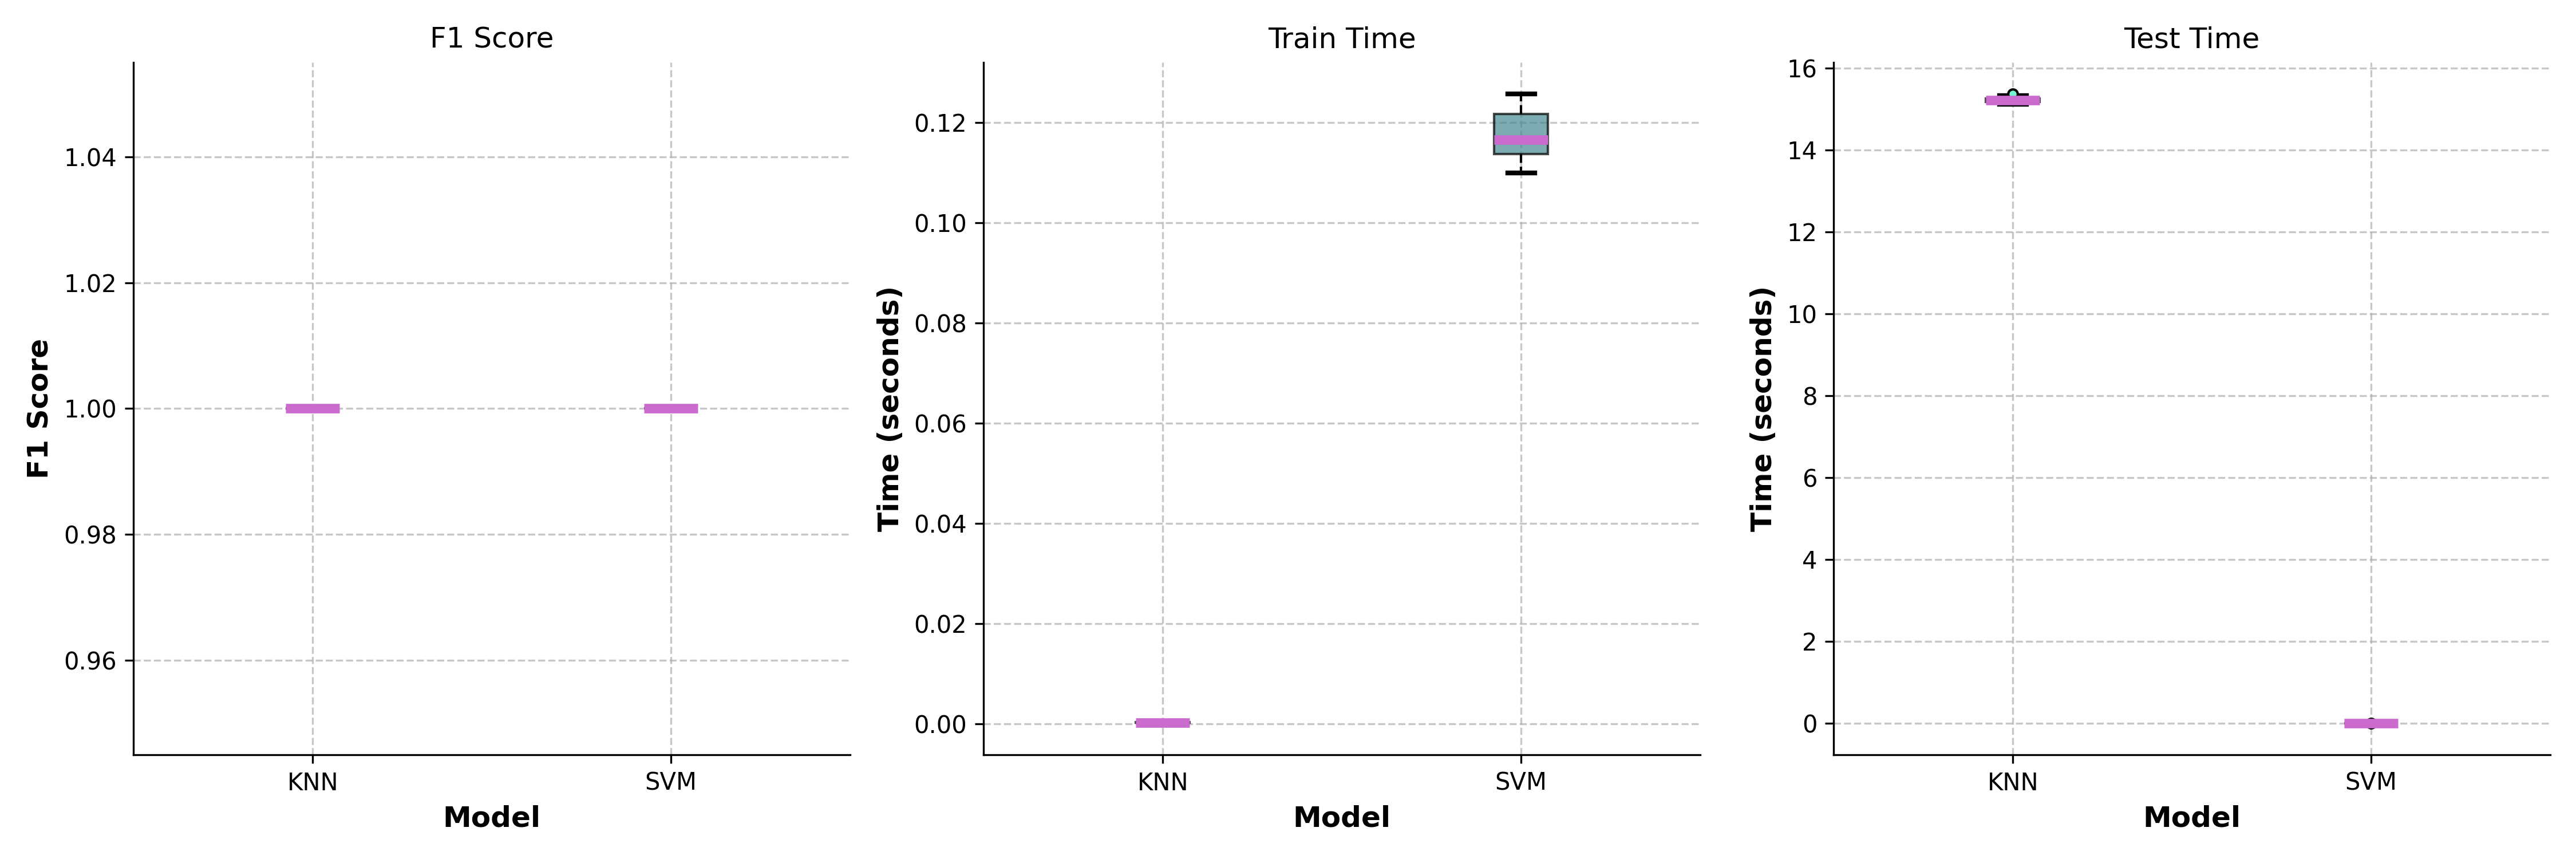
\includegraphics[width=\textwidth]{figures/model_comparison_mushroom.png}
    \caption{Comparison of the top SVM and KNN models for the Mushroom dataset}
    \label{fig:model-comparison-mushroom}
\end{figure}

\begin{figure}
    \centering
    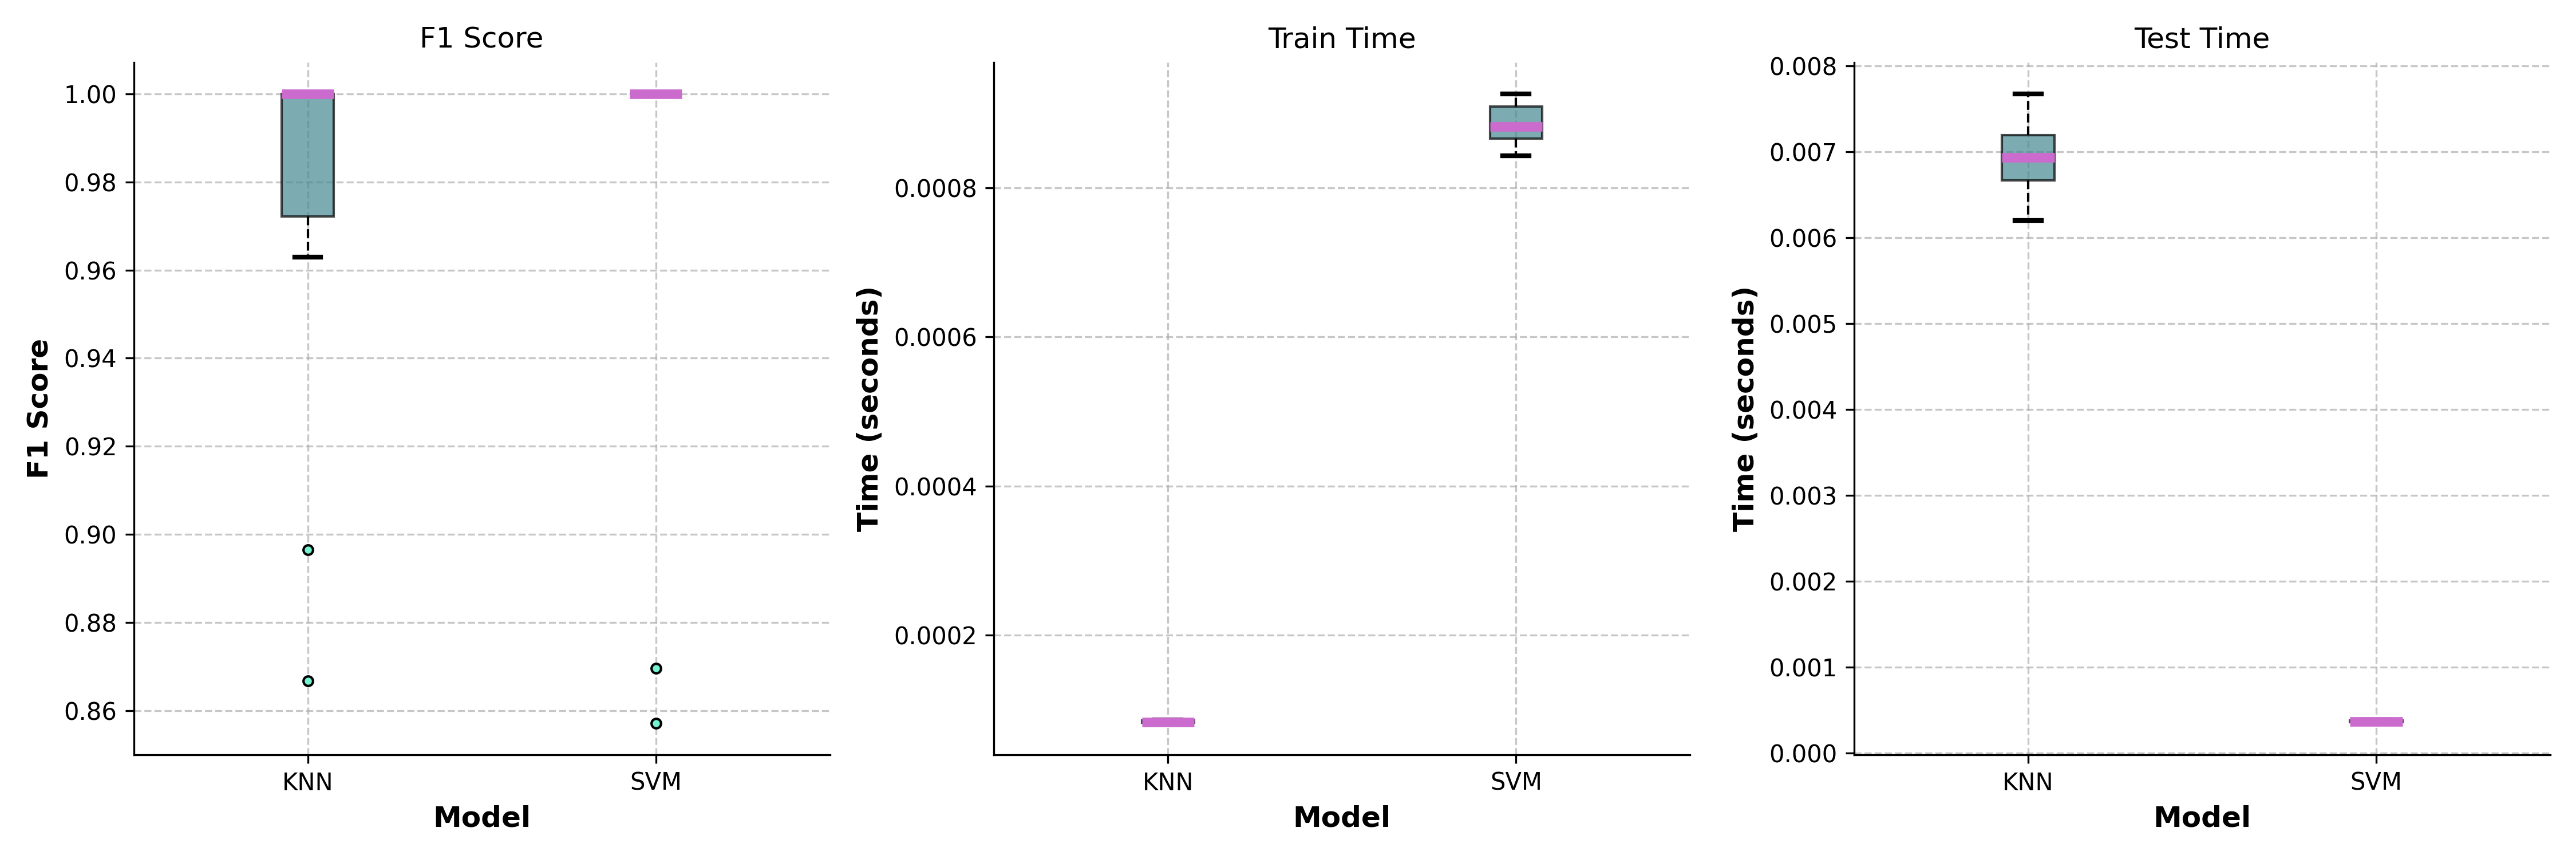
\includegraphics[width=\textwidth]{figures/model_comparison_hepatitis.png}
    \caption{Comparison of the top SVM and KNN models for the Hepatitis dataset}
    \label{fig:model-comparison-hepatitis}
\end{figure}


\paragraph{Statistical Analysis among Top Models}
We used the Wilcoxon signed-rank test (see \autoref{sec:statistical-analysis}: Statistical Analysis) to determine
the P-values indicating significant differences among the metrics F1, Train Time and Test Time for the 
top-performing SVM and KNN models.
We see that while the F1 does not vary much at all between the models, the training and testing times do vary (see \autoref{subsubsec:discussion-svm}).
This was true among both models, and the data is summarized in \autoref{tab:svm_knn_wilcoxon_comparison_hepatitis} and \autoref{tab:svm_knn_wilcoxon_comparison_mushroom}.
The comparison among these key features is shown in \autoref{fig:model-comparison-mushroom} and \autoref{fig:model-comparison-hepatitis}.

\paragraph{General Tradeoffs}
Our analysis revealed several important tradeoffs between SVM and KNN:

\begin{itemize}
    \item \textbf{Computational Complexity:} SVM typically offers faster prediction times once trained, while KNN's prediction time scales with the dataset size
    \item \textbf{Memory Requirements:} SVM models are more memory-efficient as they only store support vectors, while KNN needs to retain the entire training dataset
    \item \textbf{Interpretability:} KNN offers more intuitive interpretation of its decisions based on nearest neighbors, while SVM's decision boundaries can be more abstract
    \item \textbf{Parameter Tuning:} KNN typically requires tuning fewer parameters, making it easier to optimize for new datasets
\end{itemize}

These findings suggest that the choice between SVM and KNN should be guided by:
\begin{itemize}
    \item Dataset size and dimensionality
    \item Available computational resources
    \item Requirements for model interpretability
    \item Time constraints for model deployment and prediction
\end{itemize}

In conclusion, while both algorithms demonstrated their effectiveness, the specific characteristics of each dataset played a crucial role in determining the most suitable classifier. This reinforces the importance of thorough model evaluation and consideration of practical constraints in real-world applications.
